% this file is called up by thesis.tex
% content in this file will be fed into the main document
\ifpdf
    \graphicspath{{3/figures/PNG/}{3/figures/PDF/}{3/figures/}}
\else
    \graphicspath{{3/figures/EPS/}{3/figures/}}
\fi
\chapter{Technologie} % top level followed by section, subsection


% ----------------------- contents from here ------------------------

\section{Apache ServiceMix}
Integracja systemów informatycznych jest jednym z największych wyzwań stojących przed nowoczesnymi przedsiębiorstwami. Apache ServiceMix pomaga rozwiązać ten problem będąc bazującym na standardach, lekkim oraz stosującym paradygmat "luźnego powiązania" narzędziem. Dzięki bazowaniu na standardach w sposób drastyczny zmniejsza szanse na uzależnienie się od konkretnego dostawcy oprogramowania, przez stosowanie luźneg powiązania zmniejsza złożoność integracji. 
Jest to otwarta implementacja ESB, zbudowana w oparciu o JBI i wydana na licencji Apache, od wersji 4 ServiceMix wykorzystuje OSGi do uproszczenia podziału aplikacji na komponenty. 	
Architekturę ServiceMix'a można podzielić na 3 warstwy:
\begin{enumerate}
	\item Warstwa jądra
	\item Warstwa serwisów
	\item Warstwa aplikacji
\end{enumerate}  
\newpage
\begin{figure}[!h]
	\centering
	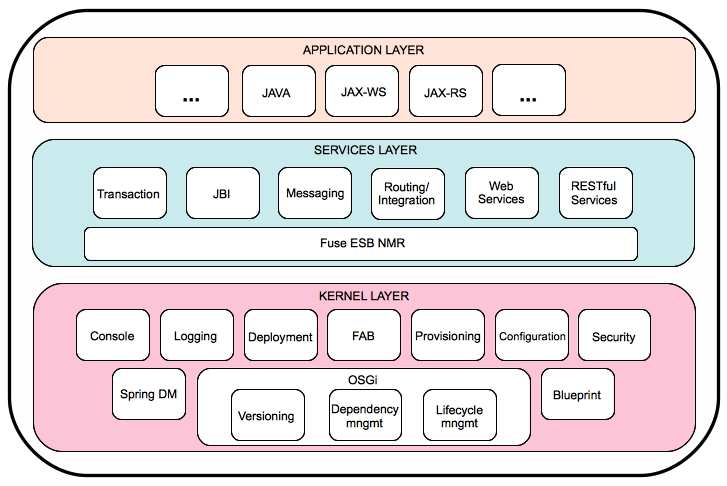
\includegraphics[scale=0.45]{ServiceMixArchitektura.jpg} 
	\caption{Architektura ServiceMix 4}
\end{figure}
Każda z tych warstw ma inne zadania i odpowiada za inne czynności.
\begin{itemize}
	\item Warstwa jądra - bazuje na Apache Karaf czyli implementacji OSGi będącą lekkim kontenerem w którym można osadzić różne komponenty i aplikacje. Warstwa ta wspólpracuje z warstwą serwisów w celu stworzenia, skoordynowania, utrzymania i zarządzania logowaniem, bezpieczeństwem oraz transakcjami. Najważniejsze funkcje dostarczane przez tą warstwę to:
	\begin{itemize}
		\item Osadzanie - umożliwia zarówno manualne jak i automatyczne osadzanie bibliotek
		\item Kontener OSGi - ServiceMix 4 wspiera 2 różne kontenery OSGi a mianowicie Eclipse Equinox i Apache Felix
		\item Wstrzykiwania zależnośći - wykorzystuje 2 różne frameworki:
			\begin{itemize}
				\item Blueprint
				\item Spring DI
			\end{itemize}   
		\item Automatyczna konfiguracja - dokonując zmian w pliku z właściwościami można dokonać zmian "w locie", bez restartowania serwera
		\item Bezpieczeństwo - framework odpowiadający za bezpieczeństwo bazuje na JAAS, dostarcza kilka różnych, odizolowanych poziomów:
			\begin{itemize}
				\item kontenera OSGi
				\item wbudowanej instancja serwisu wiadomości
				\item osadzonych instancji serwisow router'a i integracyjnego
			\end{itemize} 
		\item Logowanie - dynamiczne logowanie wspierające różne interfejsy takie jak: JCL, SLF4J, Avalon, łatwo konfigurowalne poprzez pliki z właściwościami
		\item Konsola - umożliwia zarządzanie i pełną kontrolę nad cała aplikacją
	\end{itemize}  
	\item Warstwa serwisów - 	składa się z interfejsów i klas reprezentujących wbudowane serwisy. Współpracuje z warstwą aplikacji w celu komunikacji z aplikacjami użytkowników które chcą korzystać z oferowanych serwisów. Najważniejsze funkcje dostarczane przez tą warstwę to:
	\begin{itemize}
		\item Rutowanie i integracja - bazuje na Apache Camel, umożliwia zdefiniowanie ścieżek i zaimplementowanie biznesowych wzorców w celach integracji a następnie osadzenie jako paczka OSGi
		\item Tworzenie serwisów webowych - bazzuje na Apache CXF, umożliwia, w prosty sposób, tworzenie i osadzanie jako paczka OSGi serwisów webowych implementujących API JAX-WS 
		\item Tworzenie serwisów zgodnych z wzorcem REST - bazuje na Apache CXF, umożliwia w prosty sposób, tworzenie i osadazanie jako paczka OSGi serwisów zgodnych z REST implementujących API JAX-RS
		\item Tworzenie i osadzanie jednostek i zespołów serwisów bazujących na JBI
		\item Komunikacje - udostępnia serwis wiadomości w całości zbudowany na Apache ActiveMQ, umożliwiający tworzenie i osadzanie zarówno klientów jak i nadawców wiadomości JMS
		\item Menadżer transakcji - bazuje na Apache Aries, wystawia interfejs transakcji jako serwis, umożliwia tworzenie i osadzanie zarówno aplikacji bazujących na framework'u JTA jak i na Spring'u
		\item Znormalizowany ruter wiadomości - jego główną rolą jest przekazywanie wiadomości pomiędzy różnymi aplikacjami osadzonymi w kontenerze OSGi oraz, jeżeli zachodzi taka konieczność, pomiędzy aplikacjami z OSGi a aplikacjami osadzonymi w kontenerze JBI
	\end{itemize}
	\item Warstaw aplikacji - w tym miejscu znajdując się aplikacje użytkownika, ServiceMix 4 dostarcza wielu różnych API(częściowo wymienionych w warstwie serwisów) za pomocą których aplikacje klienckie mogą łączyć się i korzystać z usług oferowanych przez serwisy działające wewnątrz kontenera
\end{itemize}

\section{IvonaTTS}
Głównym wyzwaniem stawianym przed syntezatorami mowy jest czytanie tekstu w sposób naturalny, głosem możliwie jak najbardziej podobnym do ludzkiego. Pomimo dużego postępu jaki dokonał się w tej dziedzinie w ciągu ostatnich lat, głosy oferowane przez współczesne syntezatory wciąż brzmią sztucznie, czyniąc słuchanie ich bez zmęczenia zadaniem dość trudny. IvonaTTS wykorzystuje dwie autorskie technologie, mianowicie:
\begin{itemize}
	\item BrightVoices
	\item Rapid Voice Development
\end{itemize} 
BrightVoices zapewniaja ekspresyjne, wyraziste, czyste, lektorskie brzmienie zarówno słów, zdań czy nawet całych książek. Jest ona efektem przeszło 10-letnich badań naukowych. Technologia ta korzysta z nowoczesnych algorytmów z dziedziny sztucznej inteligencji, umożliwiają one precyzyjne odzwierciedlanie ekspresji oraz różnych, nieraz bardzo indywidualnych, cech ludzkiego głosu.   \\
Rapid Voice Development w sposób znaczny przyspiesza proces tworzenia ludzkiego głosu. Pozwala także na efektywne, szybkie i precyzyjne rozpoznawianie sygnałów mowy w nagraniach lektorskich. Wszystko to jest możliwe do osiągnięcia dzięki doskonałemu modelowaniu zagadnień językowych takich jak:
\begin{itemize}
	\item akcentowanie,
	\item fonetyzacja,
	\item artykulacja,
	\item intonacja.
\end{itemize}
Według niezależnej amerykańskiej organizacji Voice Information Assiociates syntezator IvonaTTS jest najdokładniejszym spośród dostępnych na rynku komercyjnych syntezatorów. Pozostawia w tyle produkty takich firm jak Microsoft, Nuance, Loquendo czy AT\&T.
\begin{figure}[!h]
	\centering
	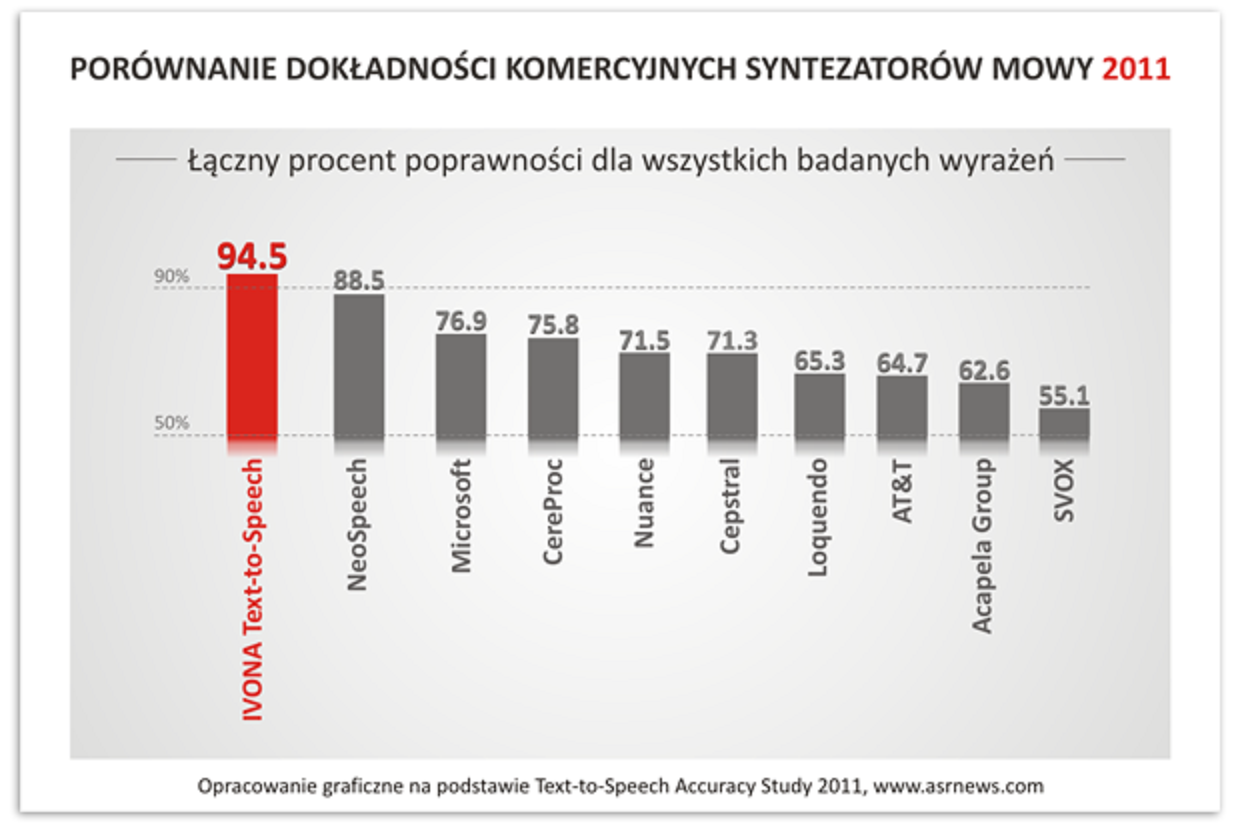
\includegraphics[scale=0.45]{IvonaWydajnosc.png} 
	\caption{Dokładność IvonaTTS w porównaniu do konkurencji}
\end{figure}

\section{FreeTTS}
FreeTTS jest syntezatorem mowy, dostępnym na licencji opensource, w całości napisanym w języku Java. Bazuje na silniku Flite stworznym i rozwijanym przez Carnegie Mellon University. Mimo swojej prostoty jego zaletami są duża wydajność, bardzo dobre radzenie sobie z językiem angielskim oraz częściowe wsparcie dla JSAPI 1.0(jako, że jest to syntezator nie wspiera częsci specyfikacji odpowiedzialnej za rozpoznawanie mowy). Dzięki temu ostatniemu w łatwy sposób umożliwia integrację z różnymi, wieloplatformowymi aplikacjami działającymi wewnątrz JVM. Przy opisywaniu tego syntezatora nie można zapomnieć o tym, że posiada dość dobrą dokumentację oraz liczne, łatwe do uruchomienia i, co bardzo ważne, działające dema. Standardowo oferuje 3 różne głosy, wszystkie w języku angielskim, umożliwia jednak rozszerzenie liczby głosów poprzez import nowych stworzonych przy pomocy narzedzi takich jak:
	\begin{itemize}
		\item FestVox,
		\item MBROLA,
		\item CMU Arctic.
	\end{itemize}    

\section{Spring}
Spring jest framework'iem przeznaczonym do tworzenia aplikacji w językach działających na JVM. Dostarcza gotowe rozwiązania dla wielu zagadnień technicznych napotykanych przez programistów. Najważniejszym elementem Spring'a jest wsparcie infratrukturalne na poziomie aplikacji. Spring skupia się na integracji elementów aplikacji, dzięki czemu programiści mogą skupić się na logice biznesowej.Framework ten można rozważać jako zbiór szablonów, większość z nich może pracować niezależnie, jakkolwiek dzięki połączeniu ich można uzyskać większą funkcjonalność. 
\newpage
Najważniejsze funkcje wspomnianych modułów to:
  \begin{itemize}
	\item Zarządzanie transakcjami - zapewnie wszechstronne, spójne wsparcie dla transakcj poprzez utworzenie odpowiedniej warstwy abstrakcji, która posiada następujące zalety:
	\begin{itemize}
		\item udostępnia generyczne, zwięzły model programowania pomiędzy różnymi interfejsami takimi jaki: JTA, JDBC, JPA itd.,
		\item bardzo łatwo integruje się z różnymi interfejsami dostępu do danych,
		\item wspiera deklaratywne zarządzanie transakcjami
	\end{itemize}
	\item Spring DI - szablon odpowiedzialny za wstrzykiwanie zależności, prawdopodobnie najbardziej popularna obecnie funkcja Spring'a, dopuszcza zarówno konfigurację za pomocą plików w formacie XML jak i przez adnotacje,
	
	\item Zaawansowane wsparcie dla programowania orientowanego aspektowo - dostarcza możliwość zaimplementowania wspólnej logiki, która następnie odwołuje się do konkretnych, potrzebnych w danej chwili modułów, umożliwia łatwe dodanie nowych modułów,
	\item Wsparcie dla elementów Java EE - dostarcza warstwę abstrakcji do pracy ze standardowymi elementami Java EE takimi jak JDBC, JTA, JMS czy JPA,
	\item Wsparcie dla testów - oferuje wsparcie dla testów jednostkowych jak i integracyjnych.
\begin{figure}[!h]
	\centering
	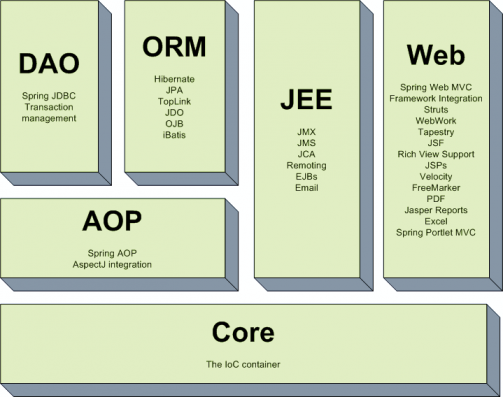
\includegraphics[scale=0.45]{springArchitektura.png} 
	\caption{Architektura Spring'a}
\end{figure}
Kolejną bardzo ważną cechą tego framework'u jest fakt, że wspiera wiele różnych platform, może działać jako osobna aplikacja, być osadzony w wielu różnych kontenerach, od najprostszego Tomcat'a do najbardziej zaawansowanych wersji WebSphere'a lub też działać w chmurze, takiej jak Heroku czy Google App Engine.  
\end{itemize}



% ---------------------------------------------------------------------------
% ----------------------- end of thesis sub-document ------------------------
% ---------------------------------------------------------------------------